\documentclass[en,license=none]{../../../eplsummary}

\usepackage{float}
\usepackage{../../../eplunits}

\graphicspath{{img/}}

\hypertitle{Computer networks}{5}{INGI}{1341}
{Gilles Peiffer}
{Olivier Bonaventure}

% TODO add some figures

\part{Principles}
\section{Connecting two hosts}

The first step when building a network,
even a worldwide network such as the Internet,
is to connect two hosts together.
In order for two hosts to exchange information,
they need to be linked by some kind of physical medium.
Various types of media have been used for this purpose:
\begin{itemize}
	\item \emph{Electrical cable}.
	Different types of cables are suitable for transmitting information:
	\begin{itemize}
		\item twisted pairs,
		which are used in the telephone network
		and in enterprise networks;
		\item coaxial cables,
		which are used in cable \textsc{TV} networks,
		but not in enterprise networks anymore.
	\end{itemize}
	Some technologies operate over the classical electrical cable.
	\item \emph{Optical fiber}.
	Optical fibers are used in networks
	when the distance between the devices is larger than one kilometer.
	There are two main types of optical fibers:
	\begin{itemize}
		\item multimode, which uses a \textsc{LED} to send signals
		over distances greater than several tens of kilometers;
		\item monomode, which uses a laser to send signals
		over distances of a few kilometers.
	\end{itemize}
	Both types can use repeaters to regenerate the signal
	and send it over another fiber.
	\item \emph{Wireless}.
	With this technology,
	a radio signal is used to encode the exchanged information.
	Modulation techniques are used
	to send information over a wireless channel.
	Some wireless networks use a laser
	that sends light pulses to a detector
	instead of a radio signal.
	These optical techniques allow to create point-to-point links,
	while radio based techniques can be used
	to build networks containing devices
	spread over a small geographical area.
\end{itemize}

\subsection{The physical layer}

The physical media explained previously can be used to exchange information,
once this information has been converted into a suitable electrical signal.
We will focus on the transmission of bits, i.e. either $0$ or $1$.

\begin{mydef}[Bit rate]
	In computer networks, the bit rate of the physical layer
	is always expressed in bits per second.
	This is in contrast with memory specifications
	which are usually expressed in bytes
	(one byte is equal to eight bits).
\end{mydef}

\subsubsection{Time-sequence diagram}

A physical transmission scheme
(interactions between communicating hosts)
can be described by using a \emph{time-sequence diagram}.
By convention, the sender is represented on the left,
and the receiver is on the right.
The middle of the diagram represents the electrical link.
Time flows from top to bottom.
To represent the transmission of a single bit,
three arrows are needed.
\begin{enumerate}
	\item The sender receives a request to transmit one bit of information.
	A \emph{primitive} is used to represent this request,
	sort of like a procedure call.
	The bit being transmitted is the only parameter.
	In the example in \figuref{timeseqdiag},
	the primitive is named \texttt{Data.request}.
	\item The dashed arrow indicates the signal's propagation time
	between the two hosts.
	Once the signal is received,
	it's interpreted and converted into a bit.
	\item The bit is delivered as a \texttt{Data.indication} primitive.
\end{enumerate}

\begin{figure}[H]
	\centering
	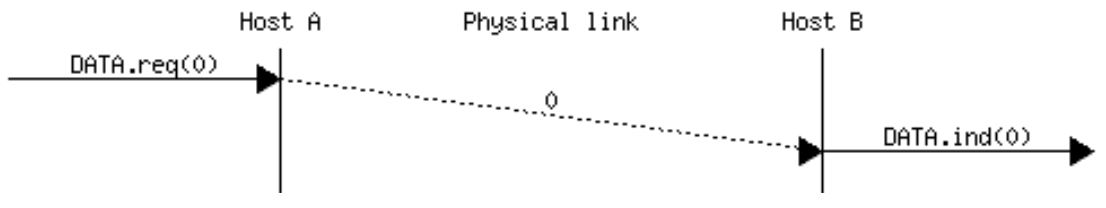
\includegraphics[width=0.5\textwidth]{timeseqdiag.png}
	\caption{A simple time-sequence diagram.}
	\label{fig:timeseqdiag}
\end{figure}

One of the problems of such a transmission scheme
is that electromagnetic interference can switch bits
while they're being transmitted
(i.e. a $0$ bit is sent but a $1$ bit is received).

With the above transmission scheme,
a bit is transmitted by setting the voltage on the electrical cable
to a specific value during some period of time.
One source of errors can be the difference in measured voltage
between the sender and the receiver.
Another reason could be that the two clocks do not operate
at exactly the same frequency.
Small differences in clock frequency imply
that bits can ``disappear'' or ``appear''
during their transmission on an electrical cable
(as in \figuref{lostbitdiag}).

\begin{figure}[H]
	\centering
	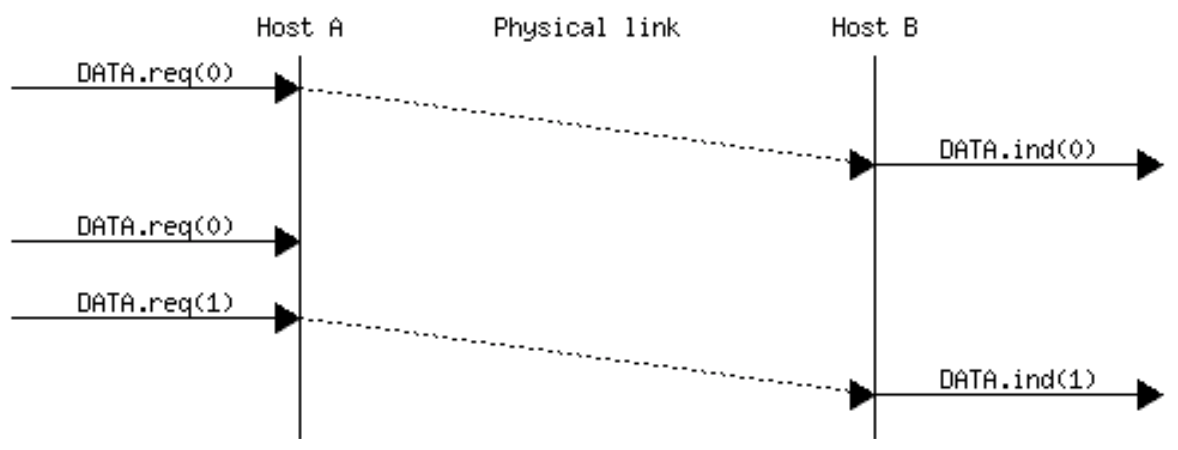
\includegraphics[width=0.5\textwidth]{lostbitdiag.png}
	\caption{Bits can ``disappear'' due to mismatched clock frequencies.}
	\label{fig:lostbitdiag}
\end{figure}

Due to these possible sources of error,
it's important to remember that the physical layer service may
\begin{itemize}
	\item \textbf{change} the value of a bit being transmitted,
	\item \textbf{deliver more (or less)} bits to the receiver
	than the bits sent by the sender.
\end{itemize}

\paragraph{Manchester encoding} Other types of encodings have been defined
to transmit information over an electrical cable.
All physical layers are able to send and receive physical symbols
that represent the values $0$ and $1$.
However, for various reasons that are outside the scope of this chapter,
several physical layers exchange other physical symbols as well.
The Manchester encoding is an encoding scheme
in which time is divided into fixed-length periods.
Each period is divided into two halves
during which different voltage levels (high or low) can be applied.
The four possible combinations make for four possible characters,
as shown in \figuref{manchester_encoding}.

\begin{figure}[H]
	\centering
	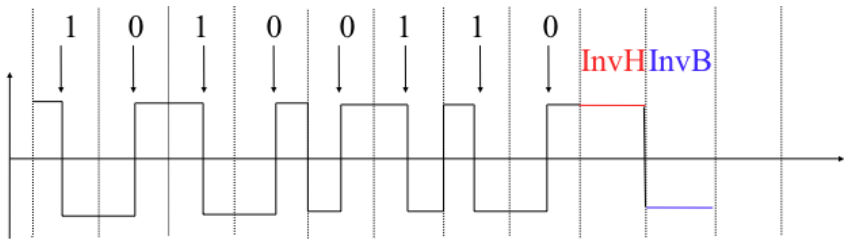
\includegraphics[width=\textwidth]{manchester_encoding.png}
	\caption{Visualisation of the Manchester encoding.
	$0$ and $1$ are regular bits,
	the InvH and InvB symbols can be used as markers
	for the beginning or end of frames.}
	\label{fig:manchester_encoding}
\end{figure}

\subsection{The datalink layer}

The physical layer is the name given
to all the functions related to the physical transmission of information.
It allows two or more entities to exchange bits
if they are connected to the same medium.
Computer networks use different layers,
where each layer provides a service that is built above the underlying layer,
and is close to the needs of the applications.
The datalink layer builds upon the service provided by the physical layer.
\bigbreak
\subsubsection{Framing}
\begin{mydef}[Frame]
	In many networks, the fundamental unit of of information
	exchanged between two hosts is called a \emph{frame}.
	A \emph{frame} is a sequence of bits
	that has a particular syntax or structure.
\end{mydef}
\begin{myrem}[Bit rate and bandwidth]
	Bit rate and bandwidth are often used
	to characterize the transmission capacity of the physical service.
	Bandwidth is defined as ``a range of radio frequencies
	which is occupied by a modulated carrier wave,
	which is assigned to a service,
	or over which a device can operate''.
	By extension, bandwidth is also used
	to represent the capacity of a communication system in bits per second.
\end{myrem}
Since the physical layer is not perfect,
transmitting and receiving frames
is not as simple as just defining a way to encode frames into bits,
or make out frames from bits.
A generic solution exists that works on any physical layer: \emph{stuffing}.
To enable a receiver to easily delineate the frame boundaries,
special bit strings serve as frame boundary markers
and encode the frames so that these special bit strings
do not appear inside the frames.
There are two variants of \emph{stuffing}:
\begin{itemize}
	\item \emph{Bit stuffing}.
	Bit stuffing reserves the $01111110$ bit string
	as the frame boundary marker
	and ensures there will never be six consecutive $1$ symbols
	transmitted by the physical layer inside a frame.
	It works as follows:
	\begin{enumerate}
		\item The sender transmits the marker, i.e. $01111110$.
		\item The sender sends all the bits of the frame
		and inserts an additional bit set to $0$
		after each sequence of five consecutive $1$ bits.
		\item The sender transmits the marker again,
		marking the end of the frame.
		\item The receiver detects the beginning of a frame
		thanks to the marker.
		\item The receiver processes the received bits,
		and if it counts five consecutive bits set to $1$,
		followed by a $0$ bit,
		that last bit is discarded.
		\item Once the receiver detects the marker again,
		it knows the frame has been received entirely.
	\end{enumerate}
	Bit stuffing increases the number of bits
	required to transmit the frame,
	with the worst case being
	a long sequence of bits set to $1$ inside the frame.
	Note that bit stuffing is vulnerable to transmission errors.
	If such an error happens,
	the frame (and possible the next)
	will not correctly be decoded by the receiver,
	but it will be able to resynchronize itself at the next valid marker.
	\item \emph{Character stuffing}.
	Character stuffing techniques
	use control characters in the \textsc{ASCII} table
	as markers to delineate frame boundaries.
	The following markers are often used:
	\textsc{DLE STX} to mark the beginning
	and \textsc{DLE ETX} to mark the end\footnote{\textsc{DLE} ($0010000$ b) for ``Data Link Escape'',
	\textsc{STX} ($0000010$ b) for ``Start of Text''
	and \textsc{ETX} ($0000011$ b) for ``End of Text''.}.
	When transmitting a frame,
	the sender adds a \textsc{DLE} character
	after each transmitted \textsc{DLE} character.
	This ensures that none of the markers
	can appear inside the transmitted frame.
	The receiver detects this
	and removes the second \textsc{DLE}
	when it receives two consecutive ones.
	Just like bit stuffing,
	character stuffing increases the length of the transmitted frames.
	The worst frame for character stuffing
	is a frame containing many \textsc{DLE} characters.
	Again, two frames can potentially be lost
	when a transmission error occurs,
	but the receiver will be able to resynchronize itself
	with the next correctly received markers.
\end{itemize}
While bit stuffing is easily implemented in hardware,
it is difficult to implement in software
given the complexity of performing bit manipulations in software.
Software implementations prefer to use character stuffing instead.

Both of these techniques allow to recover frames from a stream of bits or bytes.
The framing mechanism provides a richer service than the physical layer.
It can also be represented
using the \texttt{Data.req} and \texttt{Data.ind} primitives,
as illustrated in \figuref{stuffing_diag}.

\begin{figure}[H]
	\centering
	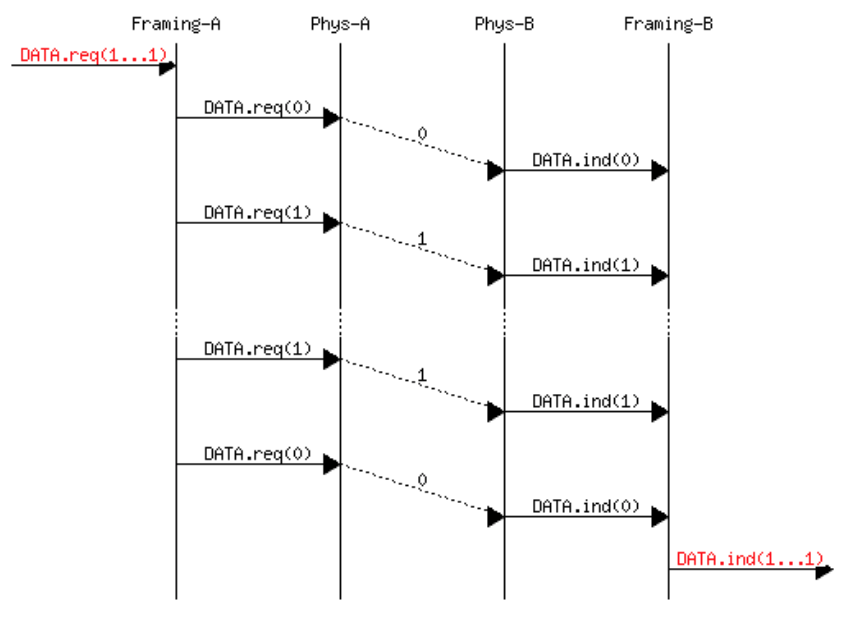
\includegraphics[width=0.4\textwidth]{stuffing_diag.png}
	\caption{Time-sequence diagram of framing,
	assuming hypothetical frames containing four useful bits
	and one bit of framing.}
	\label{fig:stuffing_diag}
\end{figure}

\subsubsection{Recovering from transmission errors}
We distinguish two types of \texttt{Data.req} and \texttt{Data.ind} primitives:
\begin{itemize}
	\item the interactions between the user and the datalink layer entity
	are represented using \texttt{Data.req} and \texttt{Data.ind};
	\item the interactions between the datalink layer entity
	and the framing sublayer
	are represented by using \texttt{send} and \texttt{recvd}.
\end{itemize}
The datalink layer entity has a buffer
to deal with \textsc{SDU}s\footnote{Service data unit,
a generic term to represent the data that is transported by a protocol.}
that have been received as a \texttt{Data.request}
but have not been sent.
It also has a buffer that deals with received frames
that haven't been processed yet.
If one of these buffers overflows,
arriving frames will be discarded,
even if they are correct.
Hence, a reliable protocol must include a feedback mechanism
that allows the receiver to inform the sender that it has processed a frame
and that another one can be sent,
regardless of transmission errors.
We need two types of frames:
\begin{itemize}
	\item \emph{data frames} carrying an \textsc{SDU};
	\item \emph{control frames} carrying an acknowledgment
	indicating the previous frames were processed correctly.
\end{itemize}
These two types can be distinguished by dividing the frame in two parts:
\begin{itemize}
	\item the \emph{header} that contains a bit
	set to $0$ in data frames and $1$ in control frames.
	\item the \emph{payload} that contains the \textsc{SDU}
	supplied by the application.
\end{itemize}
The datalink entity can then be modelled
as an \textsc{FSM}\footnote{Finite state machine.},
containing two states for the receiver and the sender (\figuref{fsm}).

\begin{figure}[H]
	\centering
	\begin{subfigure}[t]{0.45\linewidth}
		\centering
		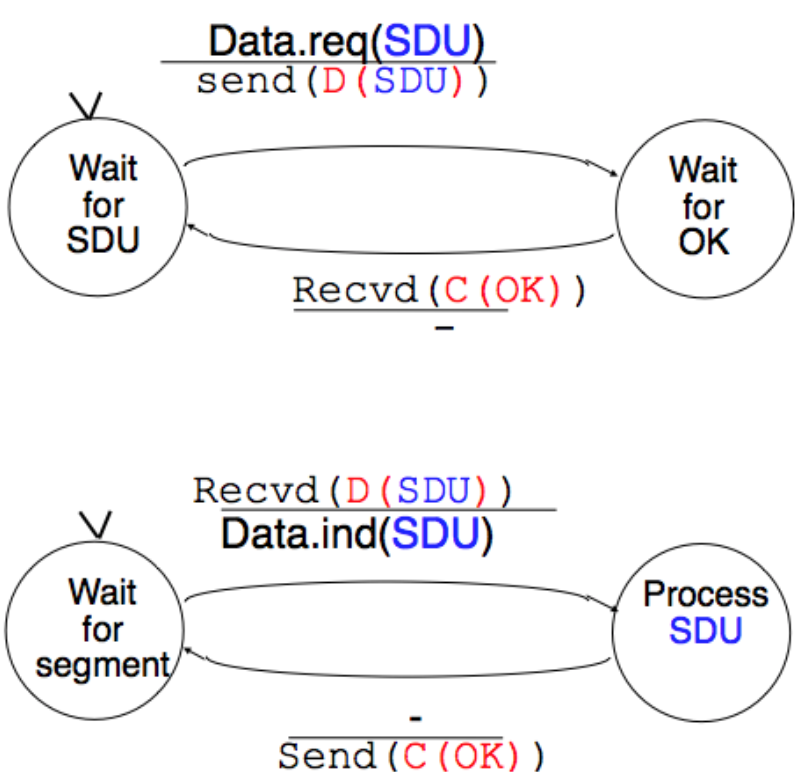
\includegraphics[width=0.6\textwidth]{fsm.png}
		\caption{\textsc{FSM} of the simplest reliable protocol,
		with the sender above and the receiver below.
		The sender has to wait for an acknowledgment
		before being able to transmit the next \textsc{SDU}.}
		\label{fig:fsm}
	\end{subfigure}
	\hfill
	\begin{subfigure}[t]{0.45\linewidth}
		\centering
		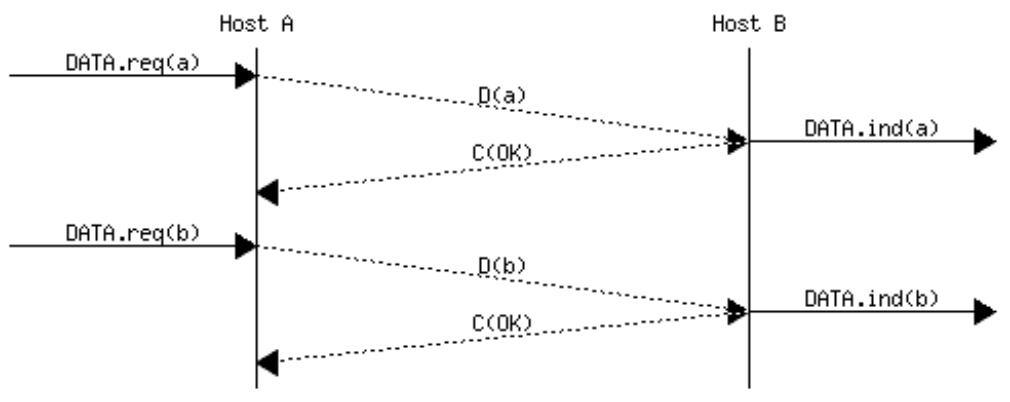
\includegraphics[width=\textwidth]{simp_rel_prot.png}
		\caption{Exchange of a few frames between two hosts.}
		\label{fig:simp_rel_prot}
	\end{subfigure}
\end{figure}

\subsubsection{Reliable data transfer on top of an imperfect link}
In the datalink layer,
we mainly have to deal with two types of transmission errors:
\begin{itemize}
	\item corrupted frames;
	\item lost or unexpected frames;
\end{itemize}
Data transmission on a physical link
can be affected by the following transmission errors:
\begin{itemize}
	\item random isolated errors
	where the value of a single bit has been modified;
	\item random burst errors
	where the values of $n$ consecutive bits have been changed;
	\item random bit creations and removals.
\end{itemize}
In order to avoid this,
we have to add \emph{redundancy} to the frames that are sent.
Information theory allows us to add redundant information
as an \emph{error detection code}.
Simply put,
the frame is sent with an error detection code,
computed by the sender, added to it.
Once the frame is received,
the receiver recomputes the error detection code
and verifies whether it matches the received one.
To understand error detection codes,
consider two devices that exchange bit strings containing $N$ bits.
To allow the receiver to detect a transmission error,
an error detection code calculates $r$ redundant bits
for each string of $N$ bits,
thus transforming the strings into strings of $N+r$ bits each.
The simplest error detection code is the parity bit.
Two types exist: even and odd parity.
With the even (resp. odd) parity scheme,
the redundant bit is chosen so that an even (resp. odd) number of bits
are set to $1$ in the transmitted string.
The receiver can easily recompute the parity of each received bit string
and discard the strings with an invalid parity.
This means that if multiple bits have been affected,
the receiver might not be able to detect the transmission error.
Another example of a (more powerful) error detection code
is a \textsc{CRC}\footnote{Cyclic redundancy check.},
which are widely used in datalink layer protocols.
\begin{myprop}[CRC]
	An $N$-bit \textsc{CRC} can detect
	\begin{itemize}
		\item all transmission errors affecting a burst
		of less than $N$ bits in the transmitted frame and
		\item all transmission errors that affect an odd number of bits.
	\end{itemize}
\end{myprop}

It is also possible to design a code
that allows the receiver to correct transmission errors,
the simplest example of which being
the \textsc{TMR}\footnote{Triple modular redundancy.},
where every bit is sent three consecutive times,
so as to allow the receiver to detect errors
and correct them by looking at the majority of bits in case an error occurs.
Other more powerful codes like the Hamming Code,
which is a clever combination of parity bits, exist.
However, these error correction schemes aren't really used in practice.

A frame is usually divided into two parts:
\begin{itemize}
	\item A \emph{header} that contains
	the fields used by the reliable protocol to ensure reliable delivery.
	The header contains a checksum or \textsc{CRC}
	that is used to detect transmission errors.
	Some headers also indicate a \emph{length field}
	with the length of the frame or the payload.
	\item A \emph{payload} that contains the user data.
\end{itemize}
The checksum is a simple error detection scheme:
both the sender and the receiver compute the arithmetic sum
of all the bytes of the frame.
Frames with an invalid checksum are discarded by the receiver.
\textsc{CRC}s have better error detection capabilities,
but require more processing power when implemented in software.
\begin{myrem}[Checksums and \textsc{CRC}s]
	Both checksums and \textsc{CRC}s are used in practice.
	The \textsc{TCP/IP} and \textsc{OSI} communities chose checksums
	(resp. the Internet checksum and the Fletcher checksum),
	while many datalink layer protocols and file formats such as
	\texttt{zip} or \texttt{png} use \textsc{CRC}s.
	It always comes down to a trade-off between error detection capabilities
	and processing power.
\end{myrem}

Since the receiver send an acknowledgment after each received data frame,
a retransmission timer is used.
The value of this retransmission timer needs to be larger
than the \textsc{RTT}\footnote{Round-trip time,
i.e. the delay between the transmission of the first bit of a data frame
to the reception of the last bit of the corresponding acknowledgment.}.
A retransmission timer is started when the sender sends a frame,
and when it expires,
the sender assumes the data segment was lost
and retransmits it (\figuref{retrans_timer}).
\begin{figure}[H]
	\centering
	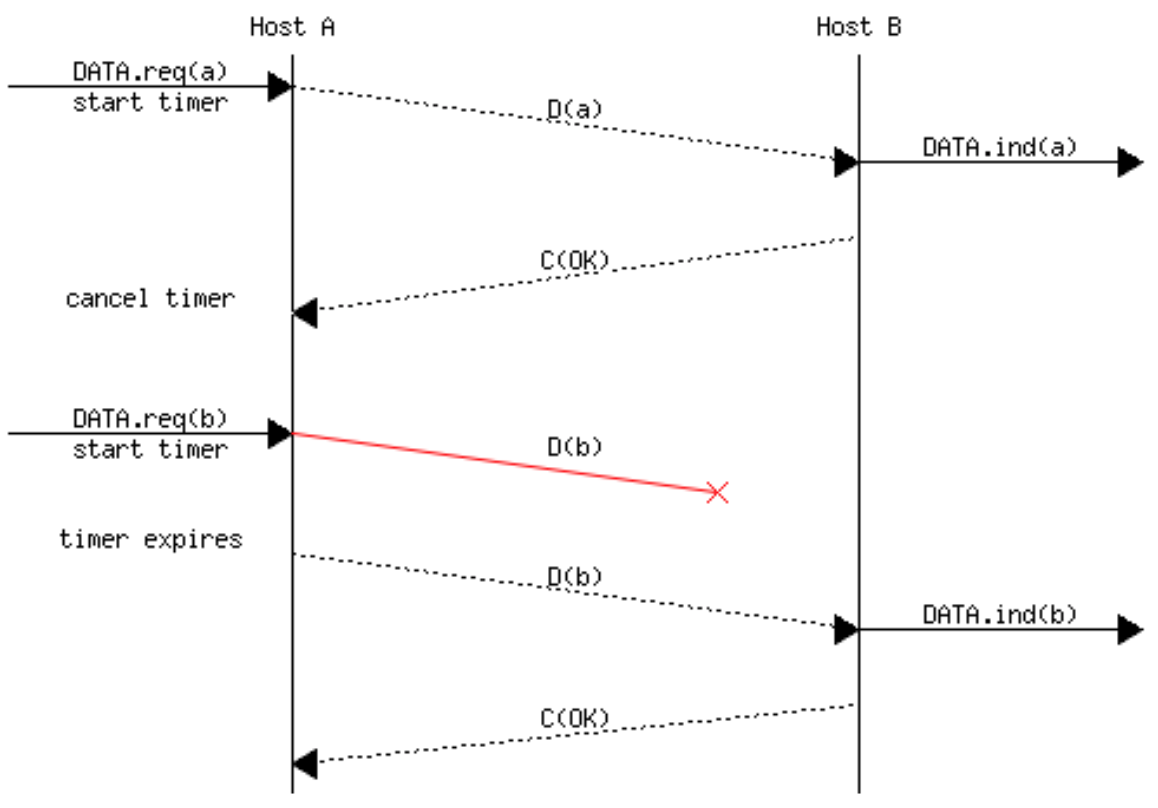
\includegraphics[width=0.4\textwidth]{retrans_timer.png}
	\caption{An example of retransmission timer expiry.}
	\label{fig:retrans_timer}
\end{figure}

However, an issue that can (and does) arise,
is the case when the acknowledgment is lost.
If this happens,
the sender will retransmit the data segment,
except that the receiver will interpret this retransmission as a new segment,
whose payload must be delivered to the user.
To solve this problem,
datalink protocols associate a seqnum\footnote{Sequence number.}
to each data frame.
This seqnum is one of the fields in the header of data frames.
We use the notation \texttt{D(x,\dots)}
to indicate a data frame whose seqnum field is set to value \texttt{x}.
The sequence number is encoded as a bit string of fixed length.
A simple reliable protocol
is \emph{Alternating bit protocol} (\textsc{ABP}).

\textsc{ABP} uses a single bit to encode the seqnum.
The sender and receiver
only require a four-state \textsc{FSM} (\figuref{abp_fsm}).

\begin{figure}[H]
	\centering
	\begin{subfigure}[t]{0.45\linewidth}
		\centering
		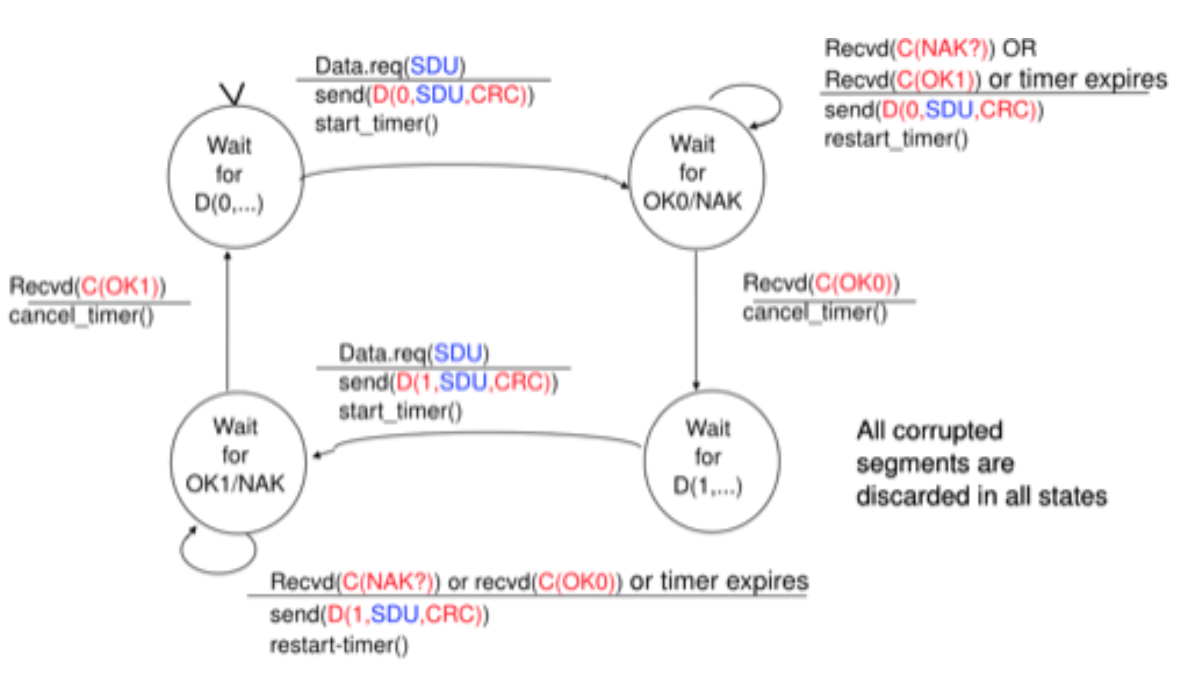
\includegraphics[width=\textwidth]{abp_sender_fsm.png}
		\caption{\textsc{ABP} sender \textsc{FSM}.
		The initial state of the sender
		is \texttt{Wait for D(0,\dots)}.
		In this state,
		the sender waits for a \texttt{Data.request}.
		The first data frame uses seqnum $0$.
		Once this is sent,
		the sender waits for an \texttt{OK0} acknowledgment.
		A frame is transmitted when the retransmission timer expires
		or when an acknowledgment with an incorrect seqnum
		has been received.}
		\label{fig:abp_sender_fsm}
	\end{subfigure}
	\hfill
	\begin{subfigure}[t]{0.45\linewidth}
		\centering
		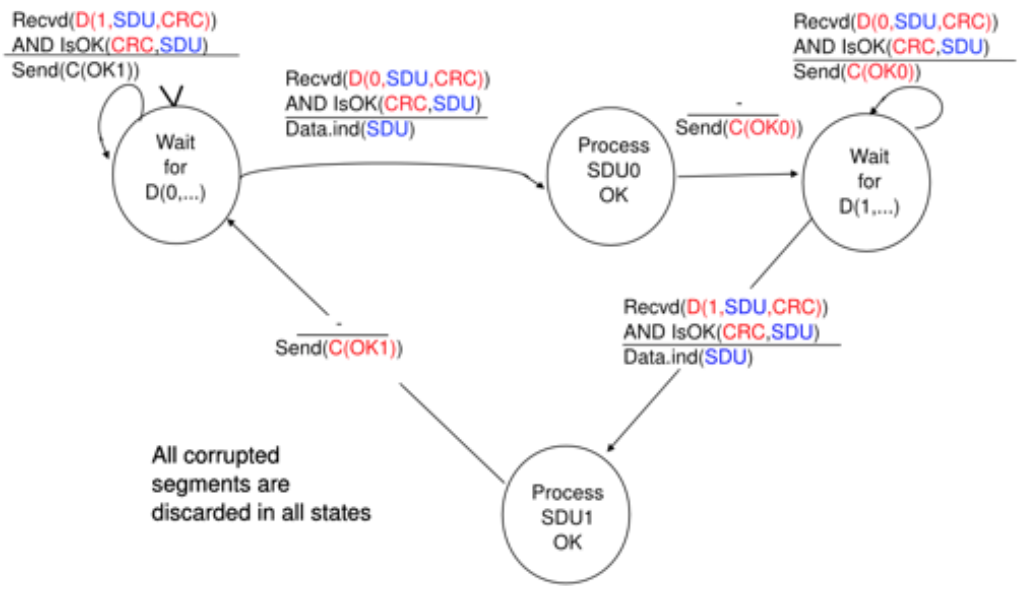
\includegraphics[width=\textwidth]{abp_receiver_fsm.png}
		\caption{\textsc{ABP} receiver \textsc{FSM}.
		The receiver first waits for \texttt{D(0,\dots)}.
		If the frame contains a correct \textsc{CRC},
		it passes the \textsc{SDU} to its user and sends \texttt{OK0}.
		If the \textsc{CRC} is invalid,
		the frame is discarded.
		The receiver then waits for \texttt{D(1,\dots)}.
		In this state,
		it may receive a duplicate \texttt{D(0,\dots)}
		or a data frame with an invalid \textsc{CRC}.
		In both cases, it returns an \texttt{OK0} frame
		to allow the sender to recover
		from the possible loss of the previous \texttt{OK0} frame.}
		\label{fig:abp_receiver_fsm}
	\end{subfigure}
	\caption{\textsc{FSM}s for the \textsc{ABP}.}
	\label{fig:abp_fsm}
\end{figure}

\textsc{ABP} can recover
from transmission errors and frame losses (shown in \figuref{abp_errors}).
However, it has an important drawback:
it has low maximum throughput.

\begin{figure}[H]
	\centering
	\begin{subfigure}[t]{0.31\linewidth}
		\centering
		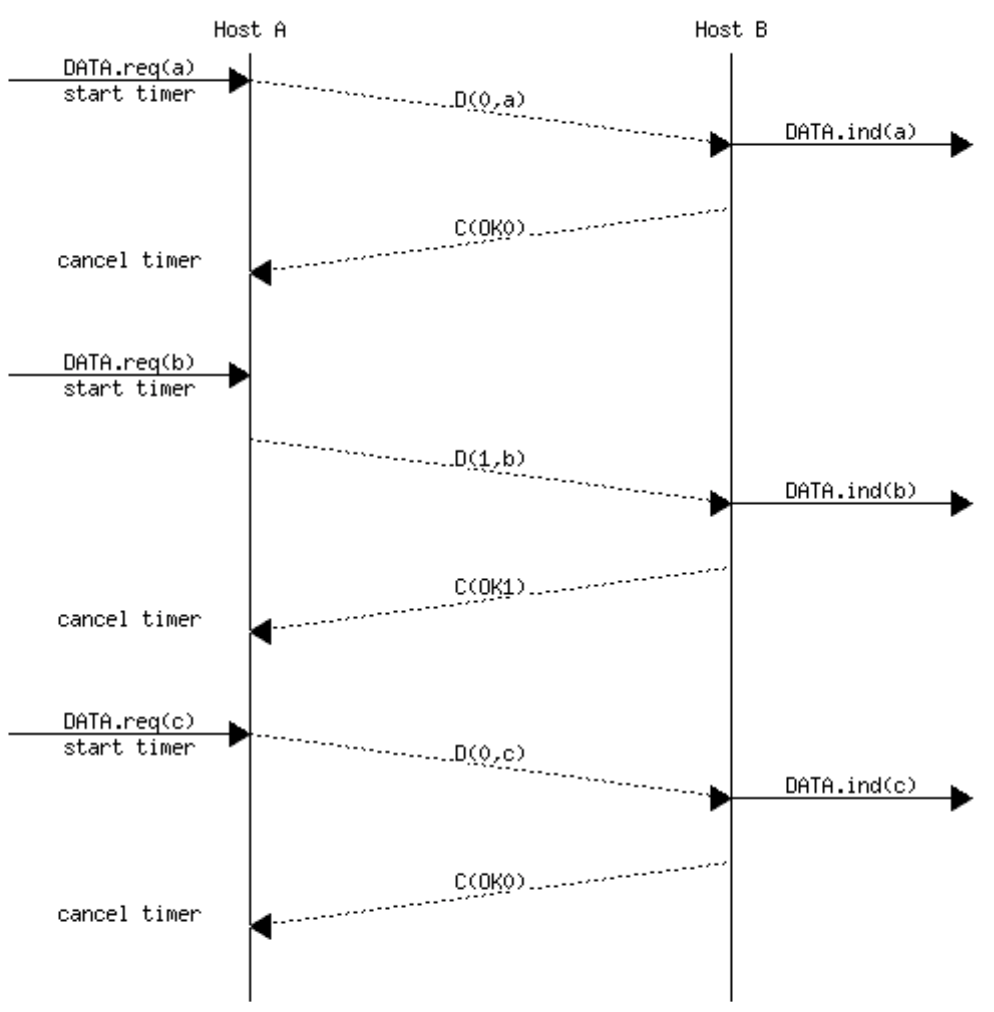
\includegraphics[width=\textwidth]{abp_success.png}
		\caption{A successful transmission with \textsc{ABP}.}
		\label{fig:abp_success}
	\end{subfigure}
	\hfill
	\begin{subfigure}[t]{0.31\linewidth}
		\centering
		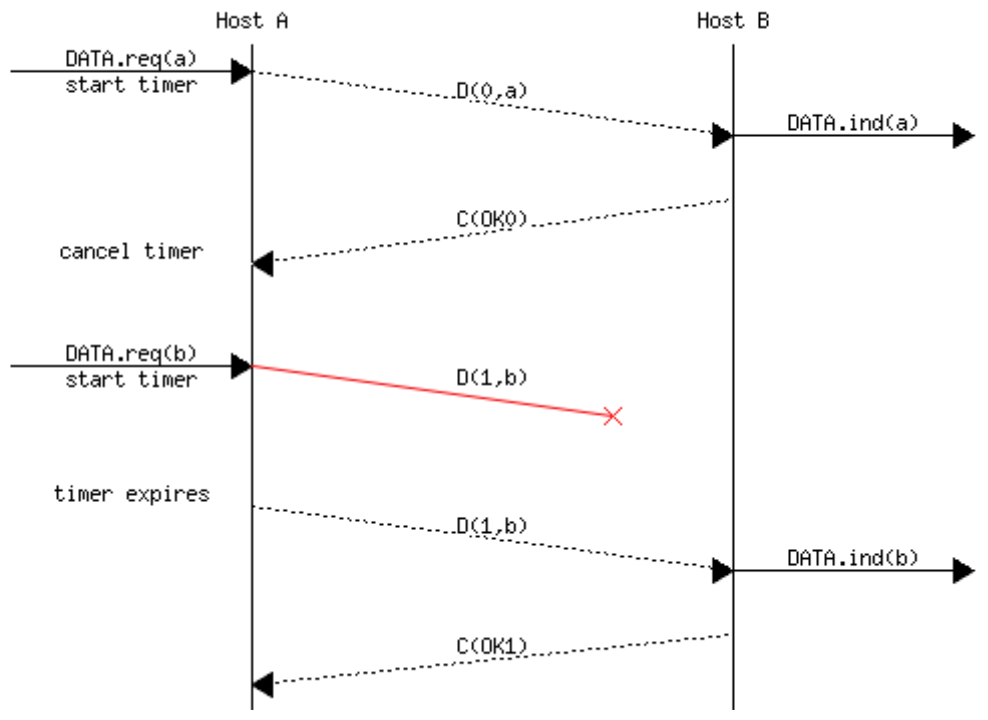
\includegraphics[width=\textwidth]{abp_error_trans.png}
		\caption{\textsc{ABP} can recover from the loss of data frames.}
		\label{fig:abp_error_trans}
	\end{subfigure}
	\hfill
	\begin{subfigure}[t]{0.31\linewidth}
		\centering
		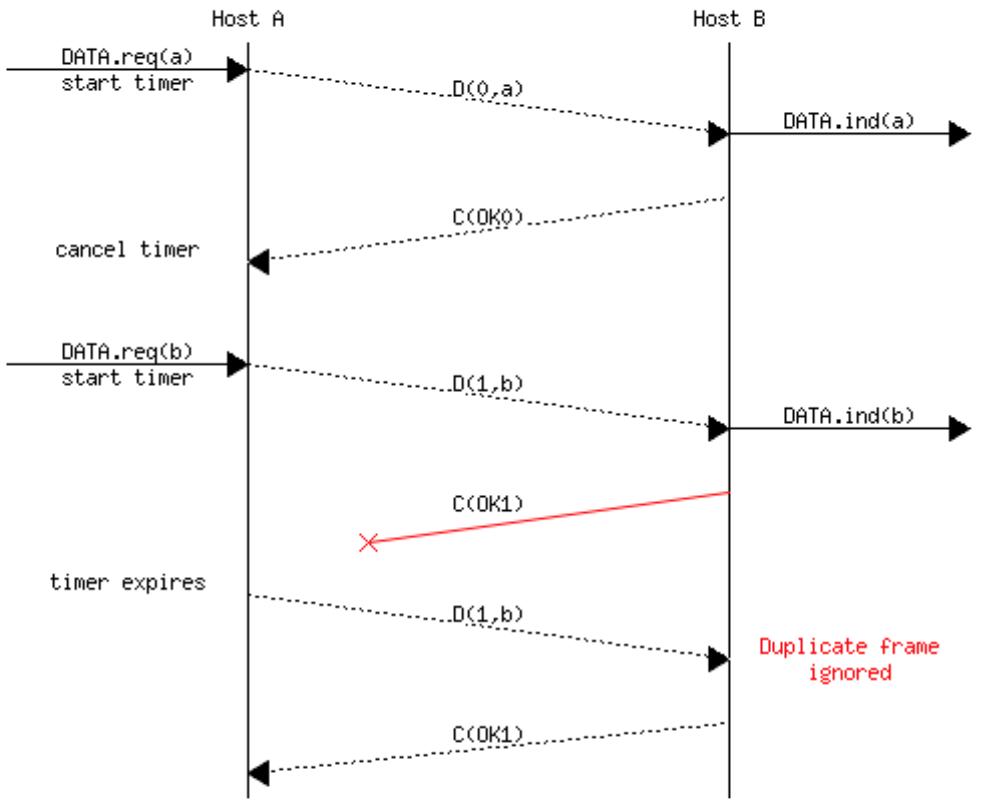
\includegraphics[width=\textwidth]{abp_error_ack.png}
		\caption{\textsc{ABP} can recover
		from the loss of control frames.}
		\label{fig:abp_error_ack}
	\end{subfigure}
	\caption{\textsc{ABP} can recover
	from the losses of data or control frames.}
	\label{fig:abp_errors}
\end{figure}
\subsubsection{Go Back $N$}
To deal with the performance limitations of \textsc{ABP},
reliable protocols rely on \emph{pipelining}.
This means a sender can send multiple consecutive frames
without having to wait for an acknowledgment after each frame.
Each frame contains a seqnum encoded in an $n$-bit field.
Pipelining can possibly overload the receiver,
which is why reliable protocols only allow
$W$ unacknowledged frames to be transmitted
before being forced to wait for an acknowledgment.
This is implemented by using a \emph{sliding window},
like the ones shown in \figuref{sliding_window}.

\begin{figure}[H]
	\centering
	\begin{subfigure}[t]{0.45\linewidth}
		\centering
		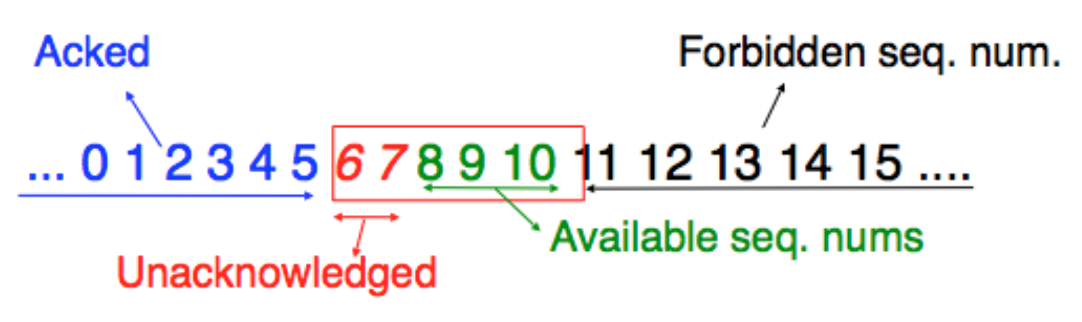
\includegraphics[width=\textwidth]{sliding_window1.png}
		\caption{An example sliding window containing $5$ segments.}
		\label{fig:sliding_window1}
	\end{subfigure}
	\hfill
	\begin{subfigure}[t]{0.45\linewidth}
		\centering
		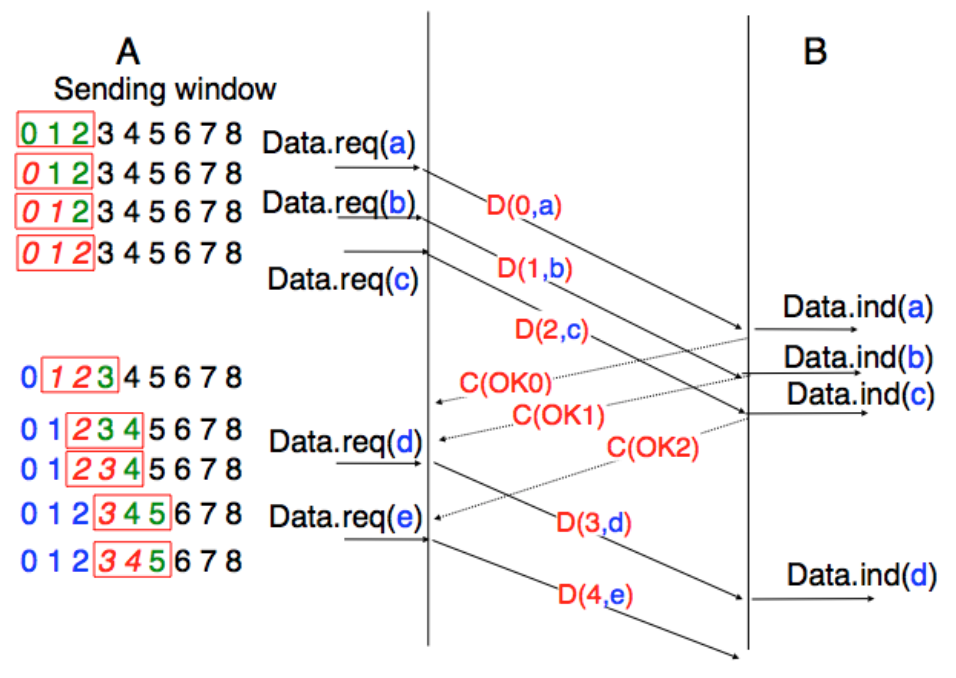
\includegraphics[width=\textwidth]{sliding_window2.png}
		\caption{An example of a sliding window of size $3$
		being used by the sender.}
		\label{fig:sliding_window2}
	\end{subfigure}
	\caption{The sliding window.}
	\label{fig:sliding_window}
\end{figure}

Note that since the headers use an $n$-bit field to encode the seqnum,
only the numbers in the interval $0$--$2^n - 1$ can be used.
This means the sliding window needs to be able to wrap.

To recover from losses,
a sliding window protocol must define
\begin{itemize}
	\item a \emph{heuristic} to detect frame losses and
	\item a \emph{retransmission strategy} to retransmit the lost frames.
\end{itemize}
The simplest such strategy is called Go Back $N$.
It works as follows:
when a receiver receives a frame,
it returns an acknowledgment containing the seqnum of
the last in-sequence frame it received.
This acknowledgment is said to be \emph{cumulative}.
This means that if the frame with seqnum $x$ is acknowledged,
then the sender knows that all previous frames were also received succesfully,
even if their acknowledgments were lost in transmission.
A sender stores a buffer of the size of the sliding window.
The frames are sent with increasing seqnums
($\mod \texttt{maxseq}$).\footnote{\texttt{maxseq} is the maximum number of different sequence numbers ($2^n$).}
Once the sending buffer is full,
it must wait for an acknowledgment.
When the sender receives an acknowledgment,
it removes all the acknowledged frames from the sending buffer,
and uses a retransmission timer to detect frame losses.
This timer is started when the first frame is sent,
and after receicing an acknowledgment,
it only restarts the timer if
there are still unacknowledged frames in the sending buffer.
When the timer expires,
all frames in the buffer are retransmitted
(and the timer is restarted again, etc.).
These possible states are summarized in \figuref{gbn_fsms}.

\begin{figure}[H]
	\centering
	\begin{subfigure}[t]{0.45\linewidth}
		\centering
		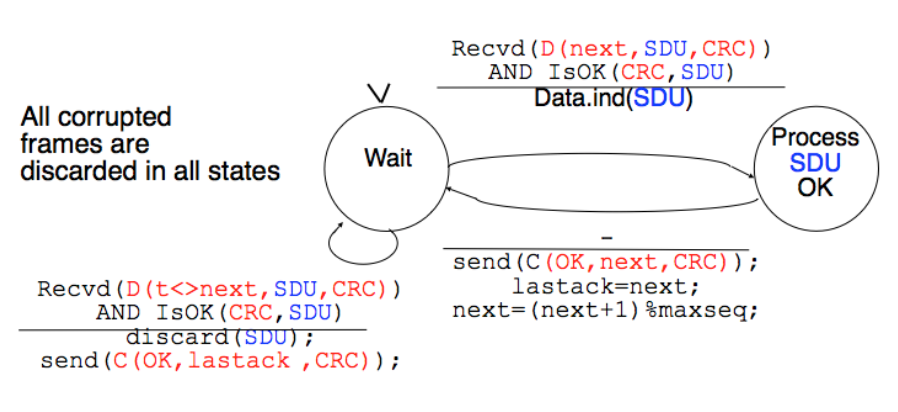
\includegraphics[width=\textwidth]{gbn_receiver_fsm.png}
		\caption{The finite state machine for a Go Back $N$ receiver.
		This receiver uses two variables:
		\texttt{lastack} and \texttt{next}.
		\texttt{next} is the next expected sequence number
		and \texttt{lastack} the sequence number
		of the last data frame that has been acknowledged.
		The receiver only accepts the frames
		that are received in sequence.}
		\label{fig:gbn_receiver_fsm}
	\end{subfigure}
	\hfill
	\begin{subfigure}[t]{0.45\linewidth}
		\centering
		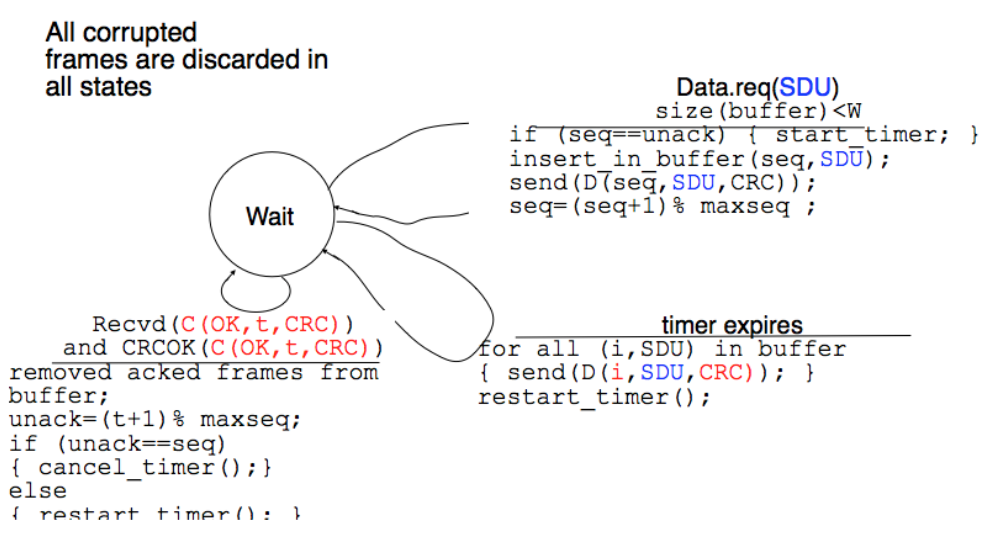
\includegraphics[width=\textwidth]{gbn_sender_fsm.png}
		\caption{The finite state machine for a Go Back $N$ sender.}
		\label{fig:gbn_sender_fsm}
	\end{subfigure}
	\caption{Finite state machines for the Go Back $N$ recovery protocol.}
	\label{fig:gbn_fsms}
\end{figure}

The operation of this protocol is illustrated in \figuref{gbn_ex}.
\begin{figure}[H]
	\centering
	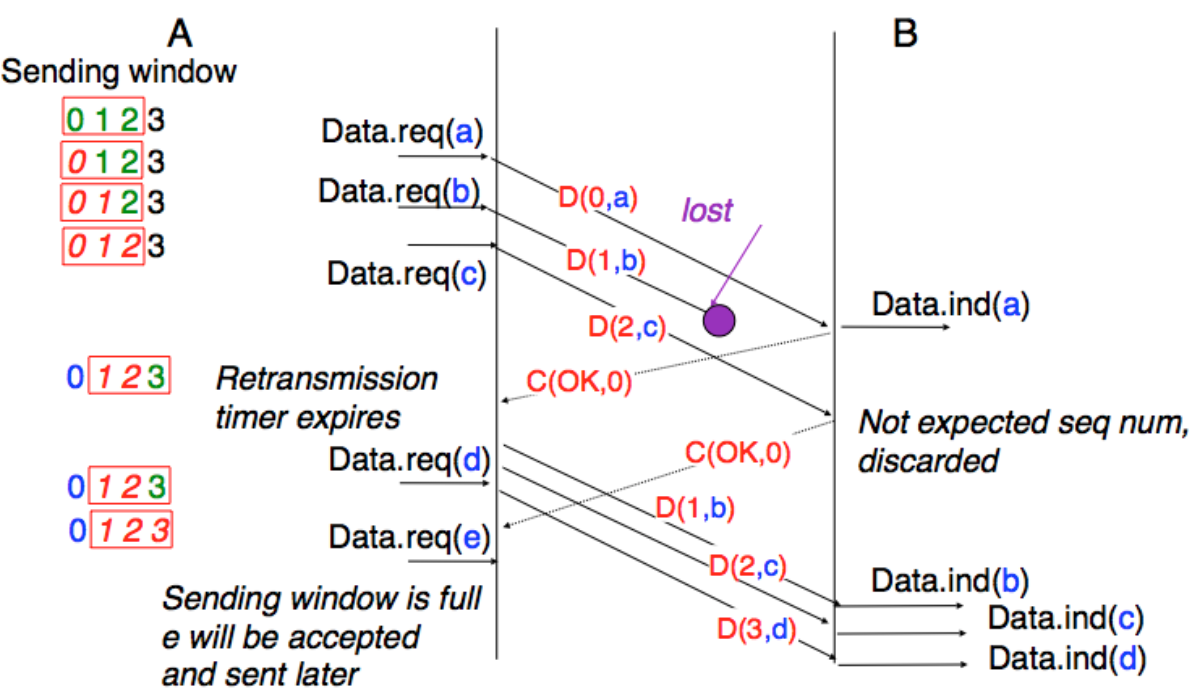
\includegraphics[width=0.6\textwidth]{gbn_ex.png}
	\caption{An example of Go Back $N$ at work.}
	\label{fig:gbn_ex}
\end{figure}

While it is easy to implement,
Go Bac $N$ also has some drawbacks:
when many frames are lost,
performance drops because out-of-sequence frames
are not accepted by the receiver and
the sender retransmits \emph{all} frames once it detects a loss.
\subsubsection{Selective repeat}
For these reasons,
selective repeat is a smarter strategy.
It has a sliding window of $W$ frames,
just like Go Back $N$,
but it also stores received out-of-frequence frames.
The selective repeat receiver discards all frames with an invalid \textsc{CRC}.
\texttt{lastack} is the last in-sequence frame received,
and it is always included in the acknowledgments that the receiver sends.
Some protocols also allow the selective repeat receiver
to acknowledge the out-of sequence frames that it has received.
This can be done by placing the list of the correctly received,
but out-of-sequence frames together with the \texttt{lastack} value.
When the receiver receives a data frame,
it first verifies whether the frame is inside its receiving window.
If yes, the frame is placed in the receive buffer.
If not, the frame is discarded and an acknowledgment with \texttt{lastack}
is sent to the sender.
The receiver then removes all consecutive frames
starting at \texttt{lastack} (if any) from the receive buffer.
The payloads of these frames are delivered to the user,
\texttt{lastack} and the receiving window are updated,
and an acknowledgment acknowledging the last frame received in sequence is sent.
\bigbreak
The selective repeat sender maintains a sending buffer
that can store up to $W$ unacknowledged frames.
These frames are sent as long as the sending buffer is not full.
Several implementations of a selective repeat sender are possible.
A simple implementation associates one retransmission timer to each frame.
The timer is started when the frame is sent
and cancelled upon reception of an acknowledgement that covers this frame.
When a retransmission timer expires,
the corresponding frame is retransmitted
and this retransmission timer is restarted.
When an acknowledgement is received,
all the frames that are covered by this acknowledgement
are removed from the sending buffer and the sliding window is updated.

\begin{figure}[H]
	\centering
	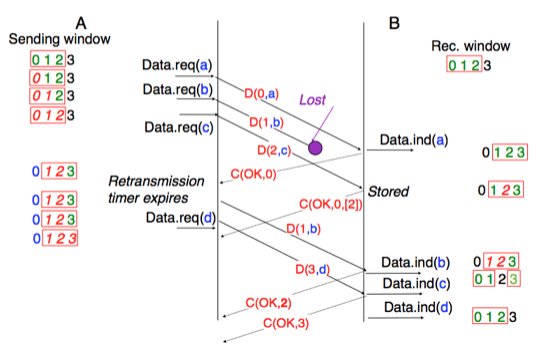
\includegraphics[width=0.6\textwidth]{selective_repeat_ex.png}
	\caption{An example of selective repeat at work.
	The figure illustrates the operation of selective repeat
	when frames are lost.
	In this figure, \texttt{C(OK,x)} is used to indicate that all frames,
	up to and including sequence number $x$ have been received correctly.
	This figure also shows selective acknowledgment,
	which the receiver telling the sender
	about correctly received,
	but out-of-sequence frames.
	The sender knows it should stop the retransmission timers
	for those frames,
	while still keeping them in the sending buffer
	until the reception of a cumulative acknowledgment.}
	\label{fig:selective_repeat_ex}
\end{figure}

\begin{myrem}[Maximum window size with Go Back $N$ and selective repeat]
	Theoretically, the maximum window size for a reliable protocol
	using $n$ bits to encode its seqnums is $2^n$.
	However, consider Go Back $N$ and that all acknowledgments are lost,
	despite the frames being received in-sequence.
	The sender will have to send all the frames again,
	and the user will receive them a second time,
	thinking they're the next batch of frames.
	This can be fixed by using $2^n-1$ instead.
	Something similar happens with selective repeat.
	To avoid this problem and have reliable delivery,
	selective repeat senders should use window of size at most $2^{n-1}$,
	so that the same frame doesn't get accepted multiple times.
\end{myrem}

Reliable protocols often need to send data in both directions.
\emph{Piggybacking} is used to avoid overhead caused by acknowledgments
by allowing the acknowledgments to be sent together with other information.
This only works when data flows in both directions.
If no data is to be sent,
the receiver will simply send a pure acknowledgment (\figuref{piggybacking}).
\begin{figure}[H]
	\centering
	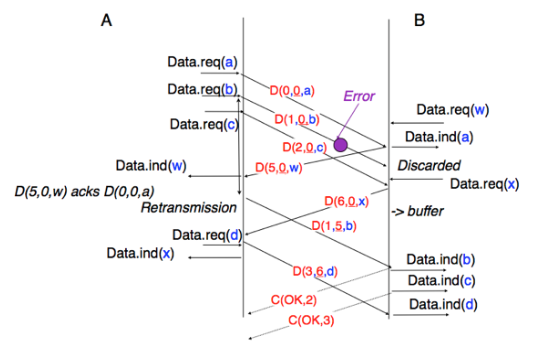
\includegraphics[width=0.6\textwidth]{piggybacking.png}
	\caption{An example of piggybacking being used.
	The bottom of the figure shows
	the receiver sending a pure acknowlegment
	when no data is to be sent in the opposite direction.}
	\label{fig:piggybacking}
\end{figure}

\section{Building a network}
When hosts aren't connected to each other by a direct physical layer link,
we need to add another layer on top of the datalink layer:
the network layer.

Its main objective is to allow end systems,
connected to different networks,
to exchange information through intermediate systems called routers.
Information is sent in packets in the network layer.

Datalink layers can be either reliable
(if the physical layer is prone to suffer from transmission errors)
or unreliable (if transmission errors are rare).
We assume here that the datalink layer service
provides an \emph{almost reliable} service.

There are two main types of datalink layers:
\begin{itemize}
	\item \emph{Point-to-point} datalink layers are used
	when there are only two communicating systems
	that are directly connected through the physical layer.
	Depending on how high the bit error ratio in the physical layer is,
	the datalink layer will be either reliable or unreliable.
	Point-to-point datalink layers can
	either connect two end systems or two routers.
	\item \textsc{LAN}s\footnote{Local area network} use
	a second type of datalink layer.
	A \textsc{LAN} is a set of communicating devices
	such that any two devices
	can directly exchange frames through the datalink layer.
\end{itemize}

Each datalink layer is characterized by a maximum frame size.
The heterogeneity in the maximum frame sizes can cause problems
when we need to exchange data between hosts
attached to different types of datalink layers.

An example network is represented in \figuref{typ_network}.
\begin{figure}[H]
	\centering
	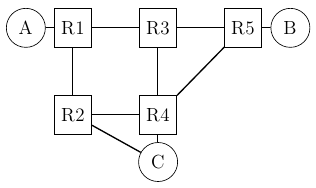
\includegraphics[width=0.4\textwidth]{typ_network.png}
	\caption{A typical network consisting of
	three end systems (or hosts, represented with circles)
	and five routers (represented with boxes).}
	\label{fig:typ_network}
\end{figure}

\begin{mydef}[End system]
	\emph{End systems}, or \emph{hosts},
	are devices which are able to send and receive data for their own usage.
	They are usually attached to the network via a single link.
	A host is \emph{multihomed} if it is equipped
	with several physical interfaces.
\end{mydef}
\begin{mydef}[Router]
	\emph{Routers}, in contrast with hosts,
	usually forward data towards its final destination.
	A router has multiple neighboring routers or hosts.
\end{mydef}

Let's analyze the operations that need to be performed to allow host $A$
in the above network to send one byte to host $B$.
Host $A$ can easily send a frame to router $R_1$ over the datalink layer.
The network layer serves to let $R_1$ know
that the data is for host $B$ and not for the router itself.

The network layer sends packets from host to host,
with intermediate routers in between.
Packets contain the information to be transmitted
as well as control information.
Each node in the network has an address
(usually a sequence of bits of fixed length).

The packet that host $A$ sends to host $B$
either contains the addresses of the source and the destination nodes,
or information that indicates the path that needs to be followed
to reach the destination.

There are two possible organisations for the network layer:
\begin{itemize}
	\item the \emph{datagram organisation} and
	\item \emph{virtual circuits}.
\end{itemize}

\subsection{The datagram organisation}
Each host is identified by its \emph{network layer address}.
Hosts create packets containing
\begin{itemize}
	\item the network layer address of the destination host;
	\item its own network layer address;
	\item the information to be sent.
\end{itemize}

Routers in the datagram organisation use \emph{hop-by-hop} forwarding.
Hence, when a router receives a packet that is not destined to itself,
it looks up the destination address in its \emph{forwarding table}.
\begin{mydef}[Forwarding table]
	A forwarding table is a data structure
	that maps each destination address
	with the outgoing interface over which this address must be forwarded.
\end{mydef}

Computing forwarding tables can be done in multiple ways,
but care must be taken so as to make sure that:
\begin{itemize}
	\item No \emph{black holes} occur.
	A black hole is when a router receives a packet with a destination
	for which it does not have an entry in its forwarding table.
	\item Packets do not get caught in an infinite loop.
\end{itemize}

The forwarding table and the format of the packets
are part of the \emph{data plane} of the network.
This data plane contains all the protocols and algorithms
that are used by hosts and routers
to create and process the packets that contain user data.
A network is also characterized by its control plane,
which contains the the protocols and algorithms
used to compute the forwarding tables.
Forwarding tables must be adapted in case of link or router failure.

\subsubsection{Computing forwarding tables}
We present three techniques for computing forwarding tables
upon the arrival of a packet.

The first technique assumes that the network topology is a tree.
This means there cannot be cycles or infinite loops.
In this technique,
routers maintain data structures called
\emph{port-address tables},
which map outgoing interfaces to destination addresses.
When the router receives a packet on a certain interface,
it learns that the source host is reachable over that interface,
and adds this to its port-address table.
If the destination address is in the router's port-address table,
it simply forwards the packet on the corresponding interface.
If not,
the packet is \emph{broadcast} over the network
(forwarded over all interfaces except the one it was received over).

This technique has two main drawbacks:
\begin{itemize}
	\item If the destination is not in the network,
	the packet gets broadcast repeatedly.
	\item Few networks have the required tree-shaped topology.
	If the network does not have this topology,
	packets can get caught in infinite loops easily.
\end{itemize}

Another technique, called \emph{source routing},
enables a destination to discover the paths
from a given source to itself,
by relying on network nodes to change some information inside packets.
We assume the data plane supports two types of packets:
data packets and control packets.

Data packets are used to exchange data,
while control packets are used to discover paths between endhosts.
When a host or router starts,
it sends a special control packet over all of its interfaces
to advertise its address to its neighbors.
When a host or node receives this control packet,
it replies with its own address.
This can also allows checking whether a neighbor is still alive.
With source routing, the data plane packets include a list of identifiers,
called a \emph{source route}.
This list is the path to be followed by the packet.
When a router receives such a packet, it forwards the packet
over the next interface in the sequence of identifiers.

Control packets contain a list that records the intermediate nodes.
When a router receives a control packet,
it looks for its own address in this \emph{record route}.
If it is included, the packet is discarded,
if not, the node adds its own address to the record route
and broadcasts the packet.
When a host receives multiple copies of the same packet,
the one that arrived first is supposed to have the best route.

Once the destination host receives the packet,
it can simply reverse the record route
and send a data packet to let the source node know the route.

\subsubsection{Flat or hierarchical addresses}
There are two ways in which addresses can be organized.
Addresses are encoded as bit strings.

Under the flat addresssing scheme,
each host and network node has a unique address.
With this scheme,
the lookup operation in the forwarding table can be implemented
with binary search if the list of addresses is sorted,
hence it has complexity $\bigoh(\lg n)$.

However, a drawback of this scheme is that
the size of the forwarding tables grows
linearly with the number of hosts and nodes in the network.

The second scheme is called hierarchical addressing,
and it divides the address into parts,
where each part narrows down the number of possible addresses.
The addressing space is divided in consecutive blocks,
then these blocks are allocated to different parts of the network.

The main advantage of hierarchical addressing over flat addressing
is the significantly reduced forwarding table size.
The drawbacks are
\begin{itemize}
	\item lookup operations become more complicated,
	\item when a host first connects to a network,
	it must contact a node to determine its own address and
	\item if a host moves, its address can change.
\end{itemize}

\subsubsection{Dealing with heterogeneous datalink layers}
When a network needs to deal with heterogeneous datalink layers,
exchanging packets becomes possible thanks to the network layer,
provided that the packet can be placed inside a datalink layer frame
before being transmitted.

If a router finds a packet that is too large
to be forwarded inside a single frame,
multiple solutions exist:
\begin{itemize}
	\item the router can send the packet back to the source host
	indicating it cannot forward packets
	longer than a certain amount of bytes;
	\item the network layer fragments the packets in two fragments
	before transmitting them,
	and then they are reassembled by the next router;
	\item the fragments are valid packets,
	and are treated as regular packets by the next routers,
	meaning the destination host receives them as two separate packets.
\end{itemize}

The first solution is simple
and does not require routers to do any fragmentation.
Hosts are more complex however,
because they need to store the packets they produce
if they pass through a narrow link.

Fragmenting the packets on a per-link basis
can minimize the transmission overhead.
Two drawbacks are that processing time
and buffer requirements on the routers are increased.
It also leads to a longer end-to-end delay since the downstream router
has to reassemble the fragments before forwarding the original packet.

The last solution is a compromise between the two others.
It has a lowed end-to-end delay
and requires less processing time and memory on the routers.

The first solution suggests using control packets
to inform the source about the reception of a long packet.
This is one of the functions of the control protocol; the others are
\begin{itemize}
	\item sending a control packet to the source
	if a router does not have a valid entry in its forwarding table;
	\item sending a control packet
	when a looping packet is detected inside the network;
	\item verifying that packets can reach a given destination.
\end{itemize}

\subsection{Virtual circuit organisation}
In a network using virtual circuits,
all hosts are identified with a network layer address.
Each packet contains a \emph{label} in its header,
which can be switched by routers.
When it receives a packet,
the router looks for this packet in its \emph{label forwarding table}
to find which interface the packet must be forwarded over.
The lookup operation has constant complexity as the table is stored as an array.
The table also indicates what the label of the outgoing packet should be set to.
The label forwarding table contains two pieces of information:
\begin{itemize}
	\item the outgoing interface for the packet;
	\item the label for the outgoing packet.
\end{itemize}
Label switching allows users to have full control
over the path followed by the packets inside the network.

Multi-Protocol Label Switching (\textsc{mpls})
is a deployed networking technology that relies on label switching.
It is more complicated than the above description however.
The control plane contains distributed algorithms,
called \emph{routing protocols},
to compute the forwarding tables that are installed on the network nodes.
Two main families of routing protocols exist:
\emph{distance vector routing} and \emph{link state routing}.

\subsection{The control plane}
One of the objectives of the control plane in the network layer
is to maintain the routing tables.

\subsubsection{Distance vector routing}
With distance vector routing,
the shortest path between hosts is computed based on \emph{metrics}
that are associated to each link.
We used \texttt{l.cost} to represent the metric
that has been configured for link \texttt{l} on a router.

Each router maintains a routing table.
The routing table \texttt{R} can be modelled as a data structure
that stores, for each known destination address \texttt{d},
the following attributes:
\begin{itemize}
	\item \texttt{R[d].link} is the outgoing link
	used to forward packets to \texttt{d};
	\item \texttt{R[d].cost} is the sum of the metrics of the links
	that compose the shortest path to reach \texttt{d};
	\item \texttt{R[d].time} is the timestamp
	of the last distance vector containing destination \texttt{d}.
\end{itemize}

A router using distance vector routing regularly sends its distance vector
over all its interfaces.
The distance vector is a summary of the router's routing table
that indicates the distance towards each known destination.

When a router receives a distance vector on link \texttt{l},
it iterates over all addresses in the distance vector.
It updates its routing table as follows:
\begin{itemize}
	\item If the distance vector contains a previously unknown address,
	the destination is inserted inside the routing table via link \texttt{l}
	and at a distance which is the sum between
	the distance in the vector and the cost of link \texttt{l}.
	\item If the address was previously known,
	the entry is updated if
	\begin{itemize}
		\item the cost of the new route is smaller than the one
		in the table (if \texttt{V[d].cost + l.cost < R[d].cost});
		\item the new route was learned over the same link
		as the current best route (\texttt{R[d].link = l}).
	\end{itemize}
	The first condition ensures that the router
	discovers the shortest path to each destination,
	while the second is used to take into account
	changes of routes in case something in the network changes.
\end{itemize}

To deal with link and router failures,
routers use the timestamp in their routing table.
Routers send their distance vector every $N$ seconds,
thus no route should have a timestamp older than $N$ seconds,
unless it is not reachable anymore.
In practice, the cutoff is at $3N$ seconds:
all routes that are older than this value
are removed when the router checks its table's timestamps every $N$ seconds.
When a router notices a route towards a destination has expired,
it associates an infinite cost to this route
and sends a distance vector to neighboring routers to inform them.
After some more waiting (typically $3N$ seconds),
the entry can be removed from the routing table.

In some situations, a problem known as ``\emph{count to infinity}'' can occur,
when two routers exchange distance vectors with increasing costs.
This problem can appear as soon as the network contains cycles.
Some protocols consider that $16$ is infinity
to mitigate the impact of counting to infinity.
This limits the metrics that operators can use
and the diameter of networks using distance vectors.

The problem occurs when a router $R_1$ advertises to another router $R_2$
a route that it has learned via $R_2$.
A solution is then a technique called \emph{split-horizon},
where routers create distance vectors that are specific to each neighbor
and only contain routes that have not been learned via this neighbor.
Another variant called \emph{split-horizon with poison-reverse}
is used as well.
In this case, routers advertise an infinite cost
for destinations that they reach
via the router to which they send the distance vector.
Not all count to infinity problems can be avoided with these techniques however.

\begin{myrem}[Forwarding tables versus routing tables]
	Routers usually maintain both a \emph{routing table}
	and a \emph{forwarding table}.
	The routing table associates a destination to an outgoing interface
	or a nexthop router, and a set of additional attributes.
	Different routing protocols store different attributes.
	Distance vector routing protocols
	will store the cost to reach the destination along the shortest path.
	The routing table is usually not directly used when forwarding packets,
	as this operation relies on a more compact data structure
	called a \emph{forwarding table}.
	This forwarding table contains
	a subset of the information found in the routing table.
	It only contains the paths that are used to forward packets,
	associating each destination to an outgoing interface or nexthop router.
\end{myrem}

\subsubsection{Link-state routing}
Link-state routing is based on routers exchanging messages
to allow each router to learn the entire network topology.

A network is modelled as a \emph{directed weighted graph}.
Each router is a node, the links are the edges in the graph
and the weights are associated according to one of these options:
\begin{itemize}
	\item unit weights;
	\item weight proportional to the propagation delay on the link;
	\item $\textnormal{weight} = \frac{C}{\textnormal{bandwidth}}$,
	where $C$ is a constant greater than the highest bandwidth.
\end{itemize}
Routers use the shortest path to reach each destination.

When a link-state router first boots,
it sends a \texttt{HELLO} message every $N$ seconds on all of its interfaces.
This message contains the router's address.
This allows all routers to know which other routers they are connected to.
\texttt{HELLO} messages are never forwarded,
and a link is considerd to have failed if
no \texttt{HELLO} message has been received from the neigboring router
for a period of $kN$ seconds.

Once a router has discovered its neighbors,
it builds \emph{link state packets} (\textsc{lsp}s),
to distribute its local links to all routers in the network.
A \textsc{lsp} contains the following information:
\begin{itemize}
	\item \texttt{LSP.router}:
	identification of the sender of the \textsc{lsp}.
	\item \texttt{LSP.age}:
	remaining lifetime of the \textsc{lsp}.
	\item \texttt{LSP.seq}:
	sequence number of the \textsc{lsp}.
	\item \texttt{LSP.links[]}:
	links advertised in the \textsc{lsp}.
	Each directed link contains the following information:
	\begin{itemize}
		\item \texttt{LSP.links[i].id}: identification of the neighbor.
		\item \texttt{LSP.links[i].cost}: cost of the link.
	\end{itemize}
\end{itemize}
The \emph{flooding} algorithm is used to distribute \textsc{lsp}s.
Each router maintains a link-state database (\textsc{lsdb})
containing the most recent \textsc{lsp} sent by each router.
When a router receives a \textsc{lsp},
it verifies whether this packet is already stored in its database.
If not, the packet is broadcast.
If it is in the database, then the packet has already been broadcast before,
and does not need to be broadcast again.

\begin{myrem}[Determining the most recent \textsc{lsp}]
	The comparison should take into account the modulo arithmetic
	used to increment the sequence numbers,
	hence divide the circle of all sequence numbers into two halves.
	Current link-state routing protocols
	use $\SI{32}{\bit}$ sequence numbers
	and include a special mechanism
	in case a sequence number reaches the maximum value.
	\textsc{lsp}s contain a checksum to deal with memory corruption,
	which can cause the algorithm to fail.

	Each router must verify the checksum
	when it receives or floods a \textsc{lsp}.
	Furthermore, each router must periodically verify the checksums
	of the \textsc{lsp}s stored in its \textsc{lsdb}.
\end{myrem}

Flooding allows \textsc{lsp}s to be distributed
to all routers inside the network without relying on routing tables.
To avoid sending the same \textsc{lsp} twice on the same link,
routers wait for a random time before forwarding \textsc{lsp}s.
In practice,
this is only done for ``refresh \textsc{lsp}s'',
as packets with new information are immediately flooded.

Link-state protocols use reliable flooding
to ensure all routers receive all \textsc{lsp}s.
To achieve this,
routers use acknowledgments and, if necessary, retransmissions.

When a link fails,
the two routers attached to this link generate and flood new \textsc{lsp}s
that no longer contain the failed link.
This might not happen at exactly the same time,
hence when other routers receive the \textsc{lsp}
of only one of the attached routers,
they still consider the link as having failed,
and remove it from the directed graph
that they compute from their \textsc{lsdb}.
When a link comes up, it can only be used
once both attached routers have advertised it in their \textsc{lsp}s.
This \emph{two-way connectivity check} also ensures that
failed routers are removed from the graph.

When a router has failed, it must be removed from the databases of all routers.
This can be done by decreasing the \texttt{age} field in each \textsc{lsp}.
Routers regularly decrement the age of the \textsc{lsp}s in their database,
and discard them once they reach zero.

To compute its forwarding table, each router computes the spanning tree
rooted at itself using Dijkstra's shortest path algorithm.
The forwarding table can be derived automatically from the spanning tree.

\section{The transport layer}
The \emph{network layer} ensures the delivery of packets on a hop-to-hop basis
through intermediate nodes.
It provides a service to the upper layer called the \emph{transport layer},
that improves the service provided by the network layer
to make it usable by applications.

Most networks use a datagram organisation and provide a simple service
which is called the \emph{connectionless service}.
The connectionless service is represented as follows on a time-sequence diagram:
a source with address \texttt{S} issues
a \texttt{Data.request} primitive (\texttt{Data.request(S, D, `M')})
containing a Service Data Unit (\textsc{sdu}) \texttt{M}
that must be delivered to destination \texttt{D},
which delivers the corresponding
\texttt{Data.indication} primitive
to the user (\texttt{Data.indication(S, D, `M')}).

A \emph{reliable connectionless service} is a service
where the service provider guarantees that all \textsc{sdu}s
submitted in \texttt{Data.request}s by a user
will eventually be delivered to their destination.
In practice, an \emph{unreliable connectionless service} is often supported.
As the transport layer is built on top of the network layer,
it is important to know the key features
of the \emph{(connectionless) network layer service}:
\begin{itemize}
	\item it can only transfer \textsc{sdu}s of \emph{limited size};
	\item it may discard \textsc{sdu}s;
	\item it may corrupt \textsc{sdu}s;
	\item it may delay, reorder of even duplicate \textsc{sdu}s.
\end{itemize}
The main cause of packet losses and errors
are the buffers used on the network nodes.

\subsection{Transport layer services}
When two applications need to communicate,
they need to structure their exchange of information.
This requires solving two problems:
\begin{itemize}
	\item How to represent information being exchanged.
	\item How to organise the interactions
	between the application and the underlying network.
	From the application's viewpoint,
	the network will appear as the \emph{transport layer service}.
	This layer provides three types of services to the applications:
	\begin{itemize}
		\item the \emph{connectionless service};
		\item the \emph{connection-oriented service};
		\item the \emph{request-response service}.
	\end{itemize}
\end{itemize}

\subsubsection{The connectionless service}
The \emph{connectionless service} is used to exchange small \textsc{sdu}s.
It can easily be built on top of the connectionless network layer service
described earlier.

\subsubsection{The connection-oriented service}
This service is used when users need to send or receive
several different and potentially large \textsc{sdu}s,
or by users who need structured exchanges.
An invocation of the \emph{connection-oriented service}
is divided into three phases:
\begin{enumerate}
	\item Establishment of a \emph{connection}.
	\begin{mydef}[Connection]
		A \emph{connection} is a temporary association
		between two users through a service provider.
		Several connections may exist at the same time
		between any pair of users.
		Connections are used to transfer \textsc{sdu}s,
		and they usually provide one bidirectional stream
		supporting the exchange of \textsc{sdu}s.
	\end{mydef}
	\item \emph{Data transfer phase}.
	The stream provided by the connection is used to transfer data.
	\item \emph{Termination} of the connection.
	Once users are done exchanging \textsc{sdu}s,
	they request termination of the connection from the provider.
\end{enumerate}

\paragraph{Connection establishment}
The establishment of a connection can be modelled using four primitives:
\begin{itemize}
	\item \texttt{Connect.request}, used to request the connection;
	\item \texttt{Connect.indication}, delivered by the provider
	to inform the destination user of the connection attempt;
	\item \texttt{Connect.response}, sent if the destination user
	accepts the connection;
	\item \texttt{Connect.confirm}, delivered by the provider
	to the user who initiated the connection.
\end{itemize}
The destination user can start sending \textsc{sdu}s
after sending a \texttt{Connect.response}.
The connection is open after sending the \texttt{Connect.confirm} primitive,
and both users can send \textsc{sdu}s at that point.

Two reasons for why a connection might fail to be established are:
\begin{itemize}
	\item The destination user may not agree to establish a connection,
	and responds to the \texttt{Connect.indication}
	with a \texttt{Disconnect.request}.
	The provider then delivers a \texttt{Disconnect.indication}
	to the initiating user.
	\item If the provider is unable to reach the destination,
	it responds to the \texttt{Connect.request}
	with a \texttt{Disconnect.indication}.
\end{itemize}

\paragraph{Data transfer phase}
Two streams are supplied to the communicating users:
\begin{itemize}
	\item the first can be used by the initiator to send \textsc{sdu}s;
	\item the second allows the responding user to send \textsc{sdu}s.
\end{itemize}

These streams can be organised in different ways:
\begin{itemize}
	\item \emph{Message-mode transfer}.
	With this organisation,
	the service prodiver guarantees that only one \texttt{Data.indication}
	will be delivered for each \texttt{Data.request}.
	\item \emph{Stream-mode transfer}.
	The service provider supplies a byte stream
	that links the two communicating users.
	\textsc{sdu}s are sent as sequences of bytes.
	The provider guarantees the order in which the bytes arrive is correct,
	but does not attempt to preserve the boundaries of the \textsc{sdu}s.
	No relation is enforced between
	the number of \texttt{Data.request}
	and \texttt{Data.indication} primitives.
	Users have to provide the mechanisms that allow the receiving user
	to separate successive \textsc{sdu}s
	in the byte stream that it receives.
\end{itemize}

\paragraph{Connection release}
Connections involve three parties (two users and a provider),
and each one of them can request connection termination.
Two types of connection release exist:
\begin{itemize}
	\item \emph{Abrupt connection release}.
	This type of release can be triggered by the provider and the users,
	and can cause losses of data.
	If the provider requests it,
	it sends a \texttt{Disconnect.indication} primitive
	to both users.
	When a user requests it,
	the user sends a \texttt{Disconnect.request(abrupt)} primitive
	to the provider, which then stops the two data streams
	and delivers the \texttt{Disconnect.indication} primitive
	to the remote user.
	\item \emph{Graceful connection release}.
	We consider both streams to be independent.
	One user issues a \texttt{Disconnect.request(graceful)} primitive
	to their provider after sending their last \texttt{Data.request},
	then closes their outbound communications.
	The provider sends all \texttt{Data.indication} primitives,
	then send the \texttt{Disconnect.indication}.
	This tells the other user that they will no longer receive \textsc{sdu}s
	over this connection,
	but are still able to issue \texttt{Data.request} primitives
	on the stream in the opposite direction,
	hence this user can close their inbound communications.

	When the user is done issuing \texttt{Data.request} primitives,
	they send a \texttt{Disconnect.request(graceful)} primitive
	to the provider,
	and close their outbound communications.
	The provider issues the necessary \texttt{Data.indication} primitives,
	then follows up with a \texttt{Disconnect.indication}.
	The other user receives this primitive
	and closes their inbound communications,
	The two streams have been released successfully,
	and the connection is completely closed.
\end{itemize}

\begin{myrem}[Reliability of the connection-oriented service]
	The connection-oriented service can only guarantee correct delivery
	of all \textsc{sdu}s
	provided that the connection has been released gracefully.
	While the connection is active, there is no such guarantee,
	as the connection may be released abruptly at any time.
\end{myrem}

\subsubsection{The request-response service}
The \emph{request-response service} is a compromise
between the connectionless service and the connection-oriented service.
It allows to efficiently exchange small amounts of information in a request
and associate it with the corresponding response.

\subsection{The transport layer}
The transport layer entity allows to deal with some issues of the network layer.

\subsubsection{Connectionless transport}
This transport service includes two additional features
on top of the connectionless network layer service.
\begin{itemize}
	\item an \emph{error detection} mechanism
	that allows to detect corrupted data;
	\item a \emph{multiplexing technique}
	that enables several applications running on one host
	to exchange information with another host.
\end{itemize}

\textsc{sdu}s are encapsulated inside \emph{segments}.
\begin{mydef}[Segment]
	The \emph{segment} is the basic unit of information
	transferred in the transport layer.
	When the transport layer entity creates a segment,
	it is encapsulated by the network layer
	into a packet with the segment as its payload and a network header.
	The packet is then encapsulated in a frame
	to be transmitted in the datalink layer.
	A segment also contains control information
	stored inside a \emph{header}.
\end{mydef}
Transport protocols rely on
checksums or \textsc{crc}s to detect transmission errors.

In order to differentiate applications running on a host,
the transport layer provides \emph{port numbers}.
Thanks to these port numbers, the transport layer
can allow applications running on one host
to exchange information with another host.

\subsubsection{Connection-oriented transport}
To support the connection-oriented service,
the transport service needs to include several mechanisms
to enrich the connectionless network layer service.

\paragraph{Connection establishment}
The connection-oriented service makes the same use of port numbers
and checksums / \textsc{crc}s as the connectionless service.
An important difference between them however is the fact that
the transport entities in the connection-oriented service
maintain some state during the lifetime of the connection.
This state is created when a connection is established,
and is removed when it is released.

Establishing a transport connection requires
defining two special control segments:
\begin{itemize}
	\item \texttt{CR}, sent by the transport entity
	that wishes to initiate a connection;
	\item \texttt{CA}, used by the remote entity to accept the connection.
\end{itemize}
Both contain port numbers that allow to identify the communicating applications.
The transport connection is said to be ``established''
once the \texttt{CA} segment has been received
(at that point, segments can be sent in both directions).
The control segments must be protected using a checksum / \textsc{crc},
and the \texttt{CR} segment can be protected using a retransmission timer.

Transport protocols also require the network layer
to bound the \emph{Maximum Segment Lifetime} (\textsc{msl}).
Segments must not remain in the network
for longer than $\textnormal{msl}$ seconds (two minutes on the Internet).
To distinguish between duplicate and new \texttt{CR}s,
a \emph{transport clock} with the following characteristics
is used inside each entity:
\begin{itemize}
	\item The clock is implemented as a $k$-bit counter,
	and its clock cycle
	is such that $2^k \times \textnormal{cycle} \gg \textnormal{MSL}$.
	The clock counter is incremented every clock cycle
	and after each connection establishment.
	\item The clock must continue to be incremented
	even if the transport entity stops or reboots.
\end{itemize}

This clock can be combined with an exchange of three segments,
called the \emph{three-way handshake},
to detect duplicates:
\begin{enumerate}
	\item The initiating transport entity sends a \texttt{CR} segment,
	with a port number and a segment number, \texttt{seq = x},
	extracted from the clock.
	The transmission is protected by a retransmission timer.
	\item The remote transport entity processes the \texttt{CR} segment,
	and creates a state for the connection attempt.
	It returns a \texttt{CA} segment
	that acknowledges the reception of the \texttt{CR} segment,
	\texttt{ack = x} and has a sequence number
	extracted from the clock, \texttt{seq = y}.
	\item The initiating entity receives the \texttt{CA} segment.
	The connection is considered to be established by the initiating entity
	and sequence numbers start their numbering at \texttt{x}.
	Before sending data, the initiating entity
	must acknowledge the received \texttt{CA} segments
	by sending another \texttt{CA} segment.
	\item The remote entity considers the transport connection
	to be established after having received the acknowledgment
	for its \texttt{CA} segment.
	Data segment numbering starts at sequence number \texttt{y}.
\end{enumerate}

This three-way handshake avoids duplicate transport connections.
Consider the following three scenarios:
\begin{itemize}
	\item If the remote entity receives an old \texttt{CR} segment,
	it replies with a \texttt{CA} segment.
	The initiating host cannot match this segment
	with a previous connection attempt,
	hence it sends a control segment, \texttt{REJECT},
	to cancel the spurious connection attempt.
	The remote entity cancels the connection attempt
	upon reception of this control segment.
	\item If the initiating entity sends a \texttt{CR} segment
	that does not reach the remote entity,
	and receives a duplicate \texttt{CA} segment
	from a previous connection attempt,
	it finds that the acknowledgment cannot be valid,
	and retransmits the \texttt{CR} segment upon expiration of the timer.
	\item If in the first scenario,
	the control segment fails to be delivered,
	and a duplicate \texttt{CA} segments reaches the remote host instead,
	the remote host realises that the acknowledgment has the wrong number
	hence it sends a control segment (\texttt{REJECT}) of its own.
\end{itemize}

\paragraph{Data transfer}
The transport protocol must include sliding windows,
retransmission timers and Go Back $N$ or selective repeat,
but cannot simply reuse techniques from the datalink layer.
The differences between the two layers are:
\begin{itemize}
	\item The transport layer must face with more variable delays.
	This happens because packets sent through a network
	do not necessarily follow the same path to their destination.
	Second, some packets may be queued in the buffers of routers,
	which can increase end-to-end delay.
	\item A network does not always deliver packets in sequence.
	\item The network may sometimes duplicate packets.
	\item The transport layer needs to include mechanisms
	to fragment and reassemble large \textsc{sdu}s.
\end{itemize}

However, both layers use checksums / \textsc{crc}s
to detect transmission errors.
Each segment contains one which is computed over the entire segment
(header and payload) by the sender and inserted in the header.
They also use sequence and acknowlegment numbers,
but in the transport layer,
the sequence number in the segment header corresponds to
the position of the first byte of the payload in the bytestream.
This allows to detect losses but also to reorder out-of-sequence segments.
It also makes fragmenting \textsc{sdu}s easier.

Sequence numbers in the transport layer are often longer
than in the datalink layer,
because they must be greater than
the number of bytes transmitted during the \textsc{msl} period.

Most transport protocols use selective repeat instead of Go Back $N$,
as transport entities should always store the segments
that it receives out-of-sequence.

A transport protocol should also allow the sender and the receiver
to adjust their window sizes,
as the memory which can be used to support
the sending or the receiving buffer of a transport connection
may change during the lifetime of the connection.

Transport protocols allow the receiver to advertise
the current size of its receiving window
in all the acknowledgments that it sends.
The sender maintains two state variables:
\begin{itemize}
	\item \texttt{swin}, the size of its sending window;
	\item \texttt{rwin}, the size of the receiving window
	advertised by the receiver.
\end{itemize}
The number of unacknowledged segments cannot be larger
than $\min(\texttt{swin}, \texttt{rwin})$.
To solve deadlock problems that can arise when the receiver advertises
a window of size $0$,
transport protocols rely on a timer called the \emph{persistence timer}.
This timer is started by the sender
whenever a receiving window of $0$ is advertised.
When the timer expires, the sender retransmits and old segment
to force a new acknowledgment.

To deal with ambiguities caused by excessive delays,
transport protocols combine large sequence number fields
with a \emph{Maximum Segment Lifetime}
to ensure segments arriving in the wrong order are handled appropriately.
If a transport protocol uses $n$ bits to encode its sequence numbers,
it cannot send more than $2^n$ segments every $\textnormal{MSL}$ seconds.

\paragraph{Connection release}
Two methods exist to release a transport connection:
\begin{itemize}
	\item Defining a new control segment (\texttt{DR}),
	and considering the connection to be released
	once this segment has been sent or received.
	This allows abrupt connection releases.
	\item Release the two directions of data transfer independently.
	When a user has sent all of their \textsc{sdu}s,
	they send a \texttt{Disconnect.request}
	for their direction of data transfer.
	The transport entity sends a control segment
	to request connection release after having sent
	all of the remaining \texttt{Data.indication} primitives.
	The remote host confirms the reception of the \texttt{DR} segment
	and the release of the corresponding direction of data transfer
	by returning an acknowlegment.
	Something similar then happens in the other direction
	once the remote host has finished sending \textsc{sdu}s.
	This constitutes a graceful connection release.
\end{itemize}
\end{document}
